\chapter{The Document Object Model}\label{dom}

\epigraphhead[30]{
\epigraph{\hspace*{-.1cm}\itshape``Too bad! Same old story! Once you've finished building your house you notice you've accidentally learned something that you really should have known—before you started.''}%
{---Friedrich Nietzsche, Beyond Good and Evil}
}\index{drawing}\index{parsing}

When you open a web page in your browser, the browser retrieves the page's \index{HTML}HTML text and parses it, much like the way our parser from \hyperref[language.parsing]{Chapter 12} parsed programs. The browser builds up a model of the document's \index{structure}structure and uses this model to draw the page on the screen.\index{live data structure}

This representation of the \index{document}document is one of the toys that a JavaScript program has available in its \index{sandbox}sandbox. It is a \index{data
structure}data
structure that you can read or modify. It acts as a \emph{live} data structure: when it's modified, the page on the screen is updated to reflect the changes.

\section{Document structure}\index{HTML!structure}

You can imagine an HTML document as a nested set of \index{box}boxes. Tags such as \lstinline`<body>` and \lstinline`</body>` enclose other \index{tag}tags, which in turn contain other tags or \index{text}text. Here's the example document from the \hyperref[browser]{previous chapter}:

\begin{lstlisting}
<!doctype html>
<html>
  <head>
    <title>My home page</title>
  </head>
  <body>
    <h1>My home page</h1>
    <p>Hello, I am Marijn and this is my home page.</p>
    <p>I also wrote a book! Read it
      <a href="http://eloquentjavascript.net">here</a>.</p>
  </body>
</html>
\end{lstlisting}
\noindent

This page has the following structure:

\vskip 1.5ex
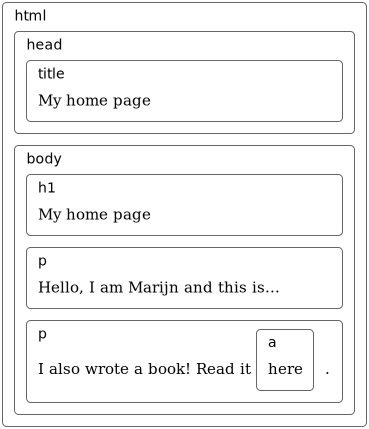
\includegraphics[width=7cm]{img/generated/html-boxes.pdf}
\vskip 1.5ex\index{Document Object Model|see{DOM}}

The data structure the browser uses to represent the document follows this shape. For each box, there is an object, which we can interact with to find out things such as what HTML tag it represents and which boxes and text it contains. This representation is called the \emph{Document Object Model}, or \index{DOM}DOM for short.\index{documentElement property}\index{head property}\index{body property}\index{html (HTML tag)}\index{body (HTML tag)}\index{head (HTML tag)}

The global binding \lstinline`document` gives us access to these objects. Its \lstinline`documentElement` property refers to the object representing the \lstinline`<html>` tag. Since every HTML document has a head and a body, it also has \lstinline`head` and \lstinline`body` properties, pointing at those elements.

\section{Trees}\index{nesting!of objects}

Think back to the \index{syntax tree}syntax trees from \hyperref[language.parsing]{Chapter 12} for a moment. Their structures are strikingly similar to the structure of a browser's document. Each \emph{\index{node}node} may refer to other nodes, \emph{children}, which in turn may have their own children. This shape is typical of nested structures where elements can contain subelements that are similar to themselves.\index{documentElement property}\index{DOM!tree}

We call a data structure a \emph{\index{tree}tree} when it has a branching structure, has no \index{cycle}cycles (a node may not contain itself, directly or indirectly), and has a single, well-defined \emph{\index{root}root}. In the case of the DOM, \lstinline`document.documentElement` serves as the root.\index{sorting}\index{data structure!tree}\index{syntax tree}

Trees come up a lot in computer science. In addition to representing recursive structures such as HTML documents or programs, they are often used to maintain sorted \index{set}sets of data because elements can usually be found or inserted more efficiently in a tree than in a flat array.\index{leaf node}\index{Egg language}

A typical tree has different kinds of \index{node}nodes. The syntax tree for \hyperref[language]{the Egg language} had identifiers, values, and application nodes. Application nodes may have children, whereas identifiers and values are \emph{leaves}, or nodes without children.\index{body property}\index{HTML!structure}

The same goes for the DOM. Nodes for \emph{\index{element}elements}, which represent HTML tags, determine the structure of the document. These can have \index{child node}child nodes. An example of such a node is \lstinline`document.body`. Some of these children can be \index{leaf node}leaf nodes, such as pieces of \index{text}text or \index{comment}comment nodes.\index{text node}\index{element}\index{ELEMENT\_NODE code}\index{COMMENT\_NODE code}\index{TEXT\_NODE code}\index{nodeType property}

Each DOM node object has a \lstinline`nodeType` property, which contains a code (number) that identifies the type of node. Elements have code 1, which is also defined as the constant property \lstinline`Node.ELEMENT_NODE`. Text nodes, representing a section of text in the document, get code 3 (\lstinline`Node.TEXT_NODE`). Comments have code 8 (\lstinline`Node.COMMENT_NODE`).

Another way to visualize our document \index{tree}tree is as follows:

\vskip 1.5ex
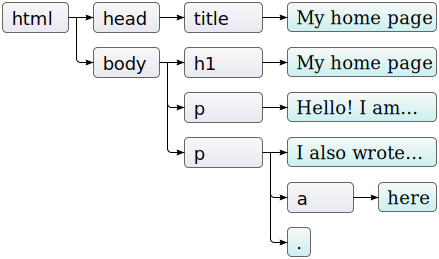
\includegraphics[width=8cm]{img/generated/html-tree.pdf}
\vskip 1.5ex

The leaves are text nodes, and the arrows indicate parent-child relationships between nodes.

\label{dom.standard}\section{The standard}\index{programming language}\index{interface!design}\index{DOM!interface}

Using cryptic numeric codes to represent node types is not a very JavaScript-like thing to do. Later in this chapter, we'll see that other parts of the DOM interface also feel cumbersome and alien. The reason for this is that the DOM wasn't designed for just JavaScript. Rather, it tries to be a language-neutral interface that can be used in other systems as well—not just for HTML but also for \index{XML}XML, which is a generic \index{data format}data format with an HTML-like syntax.\index{consistency}\index{integration}

This is unfortunate. Standards are often useful. But in this case, the advantage (cross-language consistency) isn't all that compelling. Having an interface that is properly integrated with the language you are using will save you more time than having a familiar interface across languages.\index{array-like object}\index{NodeList type}

As an example of this poor integration, consider the \lstinline`childNodes` property that element nodes in the DOM have. This property holds an array-like object, with a \lstinline`length` property and properties labeled by numbers to access the child nodes. But it is an instance of the \lstinline`NodeList` type, not a real array, so it does not have methods such as \lstinline`slice` and \lstinline`map`.\index{interface!design}\index{DOM!construction}\index{side effect}

Then there are issues that are simply poor design. For example, there is no way to create a new node and immediately add children or \index{attribute}attributes to it. Instead, you have to first create it and then add the children and attributes one by one, using side effects. Code that interacts heavily with the DOM tends to get long, repetitive, and ugly.\index{library}

But these flaws aren't fatal. Since JavaScript allows us to create our own \index{abstraction}abstractions, it is possible to design improved ways to express the operations you are performing. Many libraries intended for browser programming come with such tools.

\section{Moving through the tree}\index{pointer}

DOM nodes contain a wealth of \index{link}links to other nearby nodes. The following diagram illustrates these:

\vskip 1.5ex
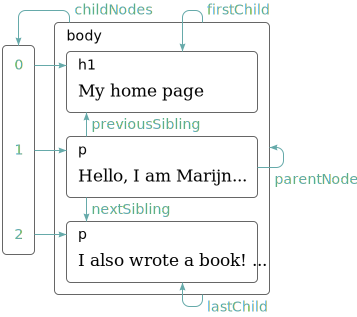
\includegraphics[width=6cm]{img/generated/html-links.pdf}
\vskip 1.5ex\index{child node}\index{parentNode property}\index{childNodes property}

Although the diagram shows only one link of each type, every node has a \lstinline`parentNode` property that points to the node it is part of, if any. Likewise, every element node (node type 1) has a \lstinline`childNodes` property that points to an \index{array-like object}array-like object holding its children.\index{firstChild property}\index{lastChild property}\index{previousSibling property}\index{nextSibling property}

In theory, you could move anywhere in the tree using just these parent and child links. But JavaScript also gives you access to a number of additional convenience links. The \lstinline`firstChild` and \lstinline`lastChild` properties point to the first and last child elements or have the value \lstinline`null` for nodes without children. Similarly, \lstinline`previousSibling` and \lstinline`nextSibling` point to adjacent nodes, which are nodes with the same parent that appear immediately before or after the node itself. For a first child, \lstinline`previousSibling` will be null, and for a last child, \lstinline`nextSibling` will be null.\index{children property}\index{text node}\index{element}

There's also the \lstinline`children` property, which is like \lstinline`childNodes` but contains only element (type 1) children, not other types of child nodes. This can be useful when you aren't interested in text nodes.\index{talksAbout function}\index{recursion}\index{nesting!of objects}

When dealing with a nested data structure like this one, recursive functions are often useful. The following function scans a document for \index{text node}text nodes containing a given string and returns \lstinline`true` when it has found one:

\label{dom.talksAbout}\begin{lstlisting}
function talksAbout(node, string) {
  if (node.nodeType == Node.ELEMENT_NODE) {
    for (let i = 0; i < node.childNodes.length; i++) {
      if (talksAbout(node.childNodes[i], string)) {
        return true;
      }
    }
    return false;
  } else if (node.nodeType == Node.TEXT_NODE) {
    return node.nodeValue.indexOf(string) > -1;
  }
}

console.log(talksAbout(document.body, "book"));
// → true
\end{lstlisting}
\noindent\index{childNodes property}\index{array-like object}\index{Array.from function}

Because \lstinline`childNodes` is not a real array, we cannot loop over it with \lstinline`for`/\lstinline`of` and have to run over the index range using a regular \lstinline`for` loop or use \lstinline`Array.from`.\index{nodeValue property}

The \lstinline`nodeValue` property of a text node holds the string of text that it represents.

\section{Finding elements}\index{DOM!querying}\index{body property}\index{hard-coding}\index{whitespace!in HTML}

Navigating these \index{link}links among parents, children, and siblings is often useful. But if we want to find a specific node in the document, reaching it by starting at \lstinline`document.body` and following a fixed path of properties is a bad idea. Doing so bakes assumptions into our program about the precise structure of the document—a structure you might want to change later. Another complicating factor is that text nodes are created even for the whitespace between nodes. The example document's \lstinline`<body>` tag does not have just three children (\lstinline`<h1>` and two \lstinline`<p>` elements) but actually has seven: those three, plus the spaces before, after, and between them.\index{search problem}\index{href attribute}\index{getElementsByTagName method}

So if we want to get the \lstinline`href` attribute of the link in that document, we don't want to say something like ``Get the second child of the sixth child of the document body''. It'd be better if we could say ``Get the first link in the document''. And we can.

\begin{lstlisting}
let link = document.body.getElementsByTagName("a")[0];
console.log(link.href);
\end{lstlisting}
\noindent\index{child node}

All element nodes have a \lstinline`getElementsByTagName` method, which collects all elements with the given tag name that are descendants (direct or indirect children) of that node and returns them as an \index{array-like
object}array-like
object.\index{id attribute}\index{getElementById method}

To find a specific \emph{single} node, you can give it an \lstinline`id` attribute and use \lstinline`document.getElementById` instead.

\begin{lstlisting}
<p>My ostrich Gertrude:</p>
<p><img id="gertrude" src="img/ostrich.png"></p>

<script>
  let ostrich = document.getElementById("gertrude");
  console.log(ostrich.src);
</script>
\end{lstlisting}
\noindent\index{getElementsByClassName method}\index{class attribute}

A third, similar method is \lstinline`getElementsByClassName`, which, like \lstinline`getElementsByTagName`, searches through the contents of an element node and retrieves all elements that have the given string in their \lstinline`class` attribute.

\section{Changing the document}\index{side effect}\index{removeChild method}\index{appendChild method}\index{insertBefore method}\index{DOM!construction}\index{DOM!modification}

Almost everything about the DOM data structure can be changed. The shape of the document tree can be modified by changing parent-child relationships. Nodes have a \lstinline`remove` method to remove them from their current parent node. To add a child node to an element node, we can use \lstinline`appendChild`, which puts it at the end of the list of children, or \lstinline`insertBefore`, which inserts the node given as the first argument before the node given as the second argument.

\begin{lstlisting}
<p>One</p>
<p>Two</p>
<p>Three</p>

<script>
  let paragraphs = document.body.getElementsByTagName("p");
  document.body.insertBefore(paragraphs[2], paragraphs[0]);
</script>
\end{lstlisting}
\noindent

A node can exist in the document in only one place. Thus, inserting paragraph \emph{Three} in front of paragraph \emph{One} will first remove it from the end of the document and then insert it at the front, resulting in \emph{Three}/\emph{One}/\emph{Two}. All operations that insert a node somewhere will, as a \index{side effect}side effect, cause it to be removed from its current position (if it has one).\index{insertBefore method}\index{replaceChild method}

The \lstinline`replaceChild` method is used to replace a child node with another one. It takes as arguments two nodes: a new node and the node to be replaced. The replaced node must be a child of the element the method is called on. Note that both \lstinline`replaceChild` and \lstinline`insertBefore` expect the \emph{new} node as their first argument.

\section{Creating nodes}\index{alt attribute}\index{img (HTML tag)}

Say we want to write a script that replaces all \index{image}images (\lstinline`<img>` tags) in the document with the text held in their \lstinline`alt` attributes, which specifies an alternative textual representation of the image.\index{createTextNode method}

This involves not only removing the images but adding a new text node to replace them. Text nodes are created with the \lstinline`document.createTextNode` method.

\begin{lstlisting}
<p>The <img src="img/cat.png" alt="Cat"> in the
  <img src="img/hat.png" alt="Hat">.</p>

<p><button onclick="replaceImages()">Replace</button></p>

<script>
  function replaceImages() {
    let images = document.body.getElementsByTagName("img");
    for (let i = images.length - 1; i >= 0; i--) {
      let image = images[i];
      if (image.alt) {
        let text = document.createTextNode(image.alt);
        image.parentNode.replaceChild(text, image);
      }
    }
  }
</script>
\end{lstlisting}
\noindent\index{text node}

Given a string, \lstinline`createTextNode` gives us a text node that we can insert into the document to make it show up on the screen.\index{live data structure}\index{getElementsByTagName method}\index{childNodes property}

The loop that goes over the images starts at the end of the list. This is necessary because the node list returned by a method like \lstinline`getElementsByTagName` (or a property like \lstinline`childNodes`) is \emph{live}. That is, it is updated as the document changes. If we started from the front, removing the first image would cause the list to lose its first element so that the second time the loop repeats, where \lstinline`i` is 1, it would stop because the length of the collection is now also 1.\index{slice method}

If you want a \emph{solid} collection of nodes, as opposed to a live one, you can convert the collection to a real array by calling \lstinline`Array.from`.

\begin{lstlisting}
let arrayish = {0: "one", 1: "two", length: 2};
let array = Array.from(arrayish);
console.log(array.map(s => s.toUpperCase()));
// → ["ONE", "TWO"]
\end{lstlisting}
\noindent\index{createElement method}

To create \index{element}element nodes, you can use the \lstinline`document.createElement` method. This method takes a tag name and returns a new empty node of the given type.\index{Popper, Karl}\index{DOM!construction}\index{elt function}

\label{dom.elt}The following example defines a utility \lstinline`elt`, which creates an element node and treats the rest of its arguments as children to that node. This function is then used to add an attribution to a quote.

\begin{lstlisting}
<blockquote id="quote">
  No book can ever be finished. While working on it we learn
  just enough to find it immature the moment we turn away
  from it.
</blockquote>

<script>
  function elt(type, ...children) {
    let node = document.createElement(type);
    for (let child of children) {
      if (typeof child != "string") node.appendChild(child);
      else node.appendChild(document.createTextNode(child));
    }
    return node;
  }

  document.getElementById("quote").appendChild(
    elt("footer", "$<—>$",
        elt("strong", "Karl Popper"),
        ", preface to the second edition of ",
        elt("em", "The Open Society and Its Enemies"),
        ", 1950"));
</script>
\end{lstlisting}
\noindent

This is what the resulting document looks like:

\vskip 1.5ex
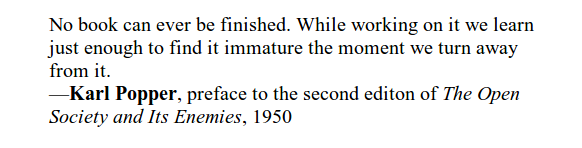
\includegraphics[width=8cm]{img/blockquote.png}
\vskip 1.5ex

\section{Attributes}\index{href attribute}\index{DOM!attributes}

Some element \index{attribute}attributes, such as \lstinline`href` for links, can be accessed through a property of the same name on the element's \index{DOM}DOM object. This is the case for most commonly used standard attributes.\index{data attribute}\index{getAttribute method}\index{setAttribute method}\index{attribute}

But HTML allows you to set any attribute you want on nodes. This can be useful because it allows you to store extra information in a document. If you make up your own attribute names, though, such attributes will not be present as properties on the element's node. Instead, you have to use the \lstinline`getAttribute` and \lstinline`setAttribute` methods to work with them.

\begin{lstlisting}
<p data-classified="secret">The launch code is 00000000.</p>
<p data-classified="unclassified">I have two feet.</p>

<script>
  let paras = document.body.getElementsByTagName("p");
  for (let para of Array.from(paras)) {
    if (para.getAttribute("data-classified") == "secret") {
      para.remove();
    }
  }
</script>
\end{lstlisting}
\noindent

It is recommended to prefix the names of such made-up attributes with \lstinline`data-` to ensure they do not conflict with any other attributes.\index{getAttribute method}\index{setAttribute method}\index{className property}\index{class attribute}

There is a commonly used attribute, \lstinline`class`, which is a \index{keyword}keyword in the JavaScript language. For historical reasons—some old JavaScript implementations could not handle property names that matched keywords—the property used to access this attribute is called \lstinline`className`. You can also access it under its real name, \lstinline`"class"`, by using the \lstinline`getAttribute` and \lstinline`setAttribute` methods.

\section{Layout}\index{layout}\index{block element}\index{inline element}\index{p (HTML tag)}\index{h1 (HTML tag)}\index{a (HTML tag)}\index{strong (HTML tag)}

You may have noticed that different types of elements are laid out differently. Some, such as paragraphs (\lstinline`<p>`) or headings (\lstinline`<h1>`), take up the whole width of the document and are rendered on separate lines. These are called \emph{block} elements. Others, such as links (\lstinline`<a>`) or the \lstinline`<strong>` element, are rendered on the same line with their surrounding text. Such elements are called \emph{inline} elements.\index{drawing}

For any given document, browsers are able to compute a layout, which gives each element a size and position based on its type and content. This layout is then used to actually draw the document.\index{border (CSS)}\index{offsetWidth property}\index{offsetHeight property}\index{clientWidth property}\index{clientHeight property}\index{dimensions}

The size and position of an element can be accessed from JavaScript. The \lstinline`offsetWidth` and \lstinline`offsetHeight` properties give you the space the element takes up in \emph{\index{pixel}pixels}. A pixel is the basic unit of measurement in the browser. It traditionally corresponds to the smallest dot that the screen can draw, but on modern displays, which can draw \emph{very} small dots, that may no longer be the case, and a browser pixel may span multiple display dots.

Similarly, \lstinline`clientWidth` and \lstinline`clientHeight` give you the size of the space \emph{inside} the element, ignoring border width.

\begin{lstlisting}
<p style="border: 3px solid red">
  I'm boxed in
</p>

<script>
  let para = document.body.getElementsByTagName("p")[0];
  console.log("clientHeight:", para.clientHeight);
  console.log("offsetHeight:", para.offsetHeight);
</script>
\end{lstlisting}
\noindent

Giving a paragraph a border causes a rectangle to be drawn around it.

\vskip 1.5ex
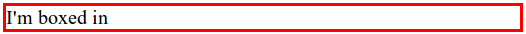
\includegraphics[width=8cm]{img/boxed-in.png}
\vskip 1.5ex\index{getBoundingClientRect method}\index{position}\index{pageXOffset property}\index{pageYOffset property}

\label{dom.boundingRect}The most effective way to find the precise position of an element on the screen is the \lstinline`getBoundingClientRect` method. It returns an object with \lstinline`top`, \lstinline`bottom`, \lstinline`left`, and \lstinline`right` properties, indicating the pixel positions of the sides of the element relative to the top left of the screen. If you want them relative to the whole document, you must add the current scroll position, which you can find in the \lstinline`pageXOffset` and \lstinline`pageYOffset` bindings.\index{offsetHeight property}\index{getBoundingClientRect method}\index{drawing}\index{laziness}\index{performance}\index{efficiency}

Laying out a document can be quite a lot of work. In the interest of speed, browser engines do not immediately re-layout a document every time you change it but wait as long as they can. When a JavaScript program that changed the document finishes running, the browser will have to compute a new layout to draw the changed document to the screen. When a program \emph{asks} for the position or size of something by reading properties such as \lstinline`offsetHeight` or calling \lstinline`getBoundingClientRect`, providing correct information also requires computing a \index{layout}layout.\index{side effect}\index{optimization}\index{benchmark}

A program that repeatedly alternates between reading DOM layout information and changing the DOM forces a lot of layout computations to happen and will consequently run very slowly. The following code is an example of this. It contains two different programs that build up a line of \emph{X} characters 2,000 pixels wide and measures the time each one takes.

\begin{lstlisting}
<p><span id="one"></span></p>
<p><span id="two"></span></p>

<script>
  function time(name, action) {
    let start = Date.now(); // Current time in milliseconds
    action();
    console.log(name, "took", Date.now() - start, "ms");
  }

  time("naive", () => {
    let target = document.getElementById("one");
    while (target.offsetWidth < 2000) {
      target.appendChild(document.createTextNode("X"));
    }
  });
  // → naive took 32 ms

  time("clever", function() {
    let target = document.getElementById("two");
    target.appendChild(document.createTextNode("XXXXX"));
    let total = Math.ceil(2000 / (target.offsetWidth / 5));
    target.firstChild.nodeValue = "X".repeat(total);
  });
  // → clever took 1 ms
</script>
\end{lstlisting}
\noindent

\section{Styling}\index{block element}\index{inline element}\index{style}\index{strong (HTML tag)}\index{a (HTML tag)}\index{underline}

We have seen that different HTML elements are drawn differently. Some are displayed as blocks, others inline. Some add styling—\lstinline`<strong>` makes its content \index{bold}bold, and \lstinline`<a>` makes it blue and underlines it.\index{img (HTML tag)}\index{default behavior}\index{style attribute}

The way an \lstinline`<img>` tag shows an image or an \lstinline`<a>` tag causes a link to be followed when it is clicked is strongly tied to the element type. But we can change the styling associated with an element, such as the text color or underline. Here is an example that uses the \lstinline`style` property:

\begin{lstlisting}
<p><a href=".">Normal link</a></p>
<p><a href="." style="color: green">Green link</a></p>
\end{lstlisting}
\noindent

The second link will be green instead of the default link color.

\vskip 1.5ex
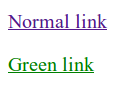
\includegraphics[width=2.2cm]{img/colored-links.png}
\vskip 1.5ex\index{border (CSS)}\index{color (CSS)}\index{CSS}\index{colon character}

A style attribute may contain one or more \emph{\index{declaration}declarations}, which are a property (such as \lstinline`color`) followed by a colon and a value (such as \lstinline`green`). When there is more than one declaration, they must be separated by \index{semicolon}semicolons, as in \lstinline`"color: red; border: none"`.\index{display (CSS)}\index{layout}

A lot of aspects of the document can be influenced by styling. For example, the \lstinline`display` property controls whether an element is displayed as a block or an inline element.

\begin{lstlisting}
This text is displayed <strong>inline</strong>,
<strong style="display: block">as a block</strong>, and
<strong style="display: none">not at all</strong>.
\end{lstlisting}
\noindent\index{hidden element}

The \lstinline`block` tag will end up on its own line since \index{block element}block elements are not displayed inline with the text around them. The last tag is not displayed at all—\lstinline`display: none` prevents an element from showing up on the screen. This is a way to hide elements. It is often preferable to removing them from the document entirely because it makes it easy to reveal them again later.

\vskip 1.5ex
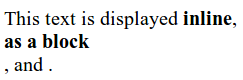
\includegraphics[width=4cm]{img/display.png}
\vskip 1.5ex\index{color (CSS)}\index{style attribute}

JavaScript code can directly manipulate the style of an element through the element's \lstinline`style` property. This property holds an object that has properties for all possible style properties. The values of these properties are strings, which we can write to in order to change a particular aspect of the element's style.

\begin{lstlisting}
<p id="para" style="color: purple">
  Nice text
</p>

<script>
  let para = document.getElementById("para");
  console.log(para.style.color);
  para.style.color = "magenta";
</script>
\end{lstlisting}
\noindent\index{camel case}\index{capitalization}\index{hyphen character}\index{font-family (CSS)}

Some style property names contain hyphens, such as \lstinline`font-family`. Because such property names are awkward to work with in JavaScript (you'd have to say \lstinline`style["font-family"]`), the property names in the \lstinline`style` object for such properties have their hyphens removed and the letters after them capitalized (\lstinline`style.fontFamily`).

\section{Cascading styles}\index{rule (CSS)}\index{style (HTML tag)}\index{Cascading Style Sheets|see{CSS}}\index{style sheet|see{CSS}}

The styling system for HTML is called \index{CSS}CSS, for \emph{Cascading Style Sheets}. A \emph{style sheet} is a set of rules for how to style elements in a document. It can be given inside a \lstinline`<style>` tag.

\begin{lstlisting}
<style>
  strong {
    font-style: italic;
    color: gray;
  }
</style>
<p>Now <strong>strong text</strong> is italic and gray.</p>
\end{lstlisting}
\noindent\index{rule (CSS)}\index{font-weight (CSS)}\index{overlay}

The \emph{\index{cascading}cascading} in the name refers to the fact that multiple such rules are combined to produce the final style for an element. In the example, the default styling for \lstinline`<strong>` tags, which gives them \lstinline`font-weight: bold`, is overlaid by the rule in the \lstinline`<style>` tag, which adds \lstinline`font-style` and \lstinline`color`.\index{style (HTML tag)}\index{style attribute}

When multiple rules define a value for the same property, the most recently read rule gets a higher \index{precedence}precedence and wins. So if the rule in the \lstinline`<style>` tag included \lstinline`font-weight: normal`, contradicting the default \lstinline`font-weight` rule, the text would be normal, \emph{not} bold. Styles in a \lstinline`style` attribute applied directly to the node have the highest precedence and always win.\index{uniqueness}\index{class attribute}\index{id attribute}

It is possible to target things other than \index{tag}tag names in CSS rules. A rule for \lstinline`.abc` applies to all elements with \lstinline`"abc"` in their \lstinline`class` attribute. A rule for \lstinline`#xyz` applies to the element with an \lstinline`id` attribute of \lstinline`"xyz"` (which should be unique within the document).

\begin{lstlisting}
.subtle {
  color: gray;
  font-size: 80%;
}
#header {
  background: blue;
  color: white;
}
/* p elements with id main and with classes a and b */
p#main.a.b {
  margin-bottom: 20px;
}
\end{lstlisting}
\noindent\index{rule (CSS)}

The \index{precedence}precedence rule favoring the most recently defined rule applies only when the rules have the same \emph{\index{specificity}specificity}. A rule's specificity is a measure of how precisely it describes matching elements, determined by the number and kind (tag, class, or ID) of element aspects it requires. For example, a rule that targets \lstinline`p.a` is more specific than rules that target \lstinline`p` or just \lstinline`.a` and would thus take precedence over them.\index{direct child node}

The notation \lstinline`p > a {…}` applies the given styles to all \lstinline`<a>` tags that are direct children of \lstinline`<p>` tags. Similarly, \lstinline`p a {…}` applies to all \lstinline`<a>` tags inside \lstinline`<p>` tags, whether they are direct or indirect children.

\section{Query selectors}\index{complexity}\index{CSS}

We won't be using style sheets all that much in this book. Understanding them is helpful when programming in the browser, but they are complicated enough to warrant a separate book.\index{domain-specific language}\index{DOM!querying}

The main reason I introduced \emph{\index{selector}selector} syntax—the notation used in style sheets to determine which elements a set of styles apply to—is that we can use this same mini-language as an effective way to find DOM elements.\index{querySelectorAll method}\index{NodeList type}

The \lstinline`querySelectorAll` method, which is defined both on the \lstinline`document` object and on element nodes, takes a selector string and returns a \lstinline`NodeList` containing all the elements that it matches.

\begin{lstlisting}
<p>And if you go chasing
  <span class="animal">rabbits</span></p>
<p>And you know you're going to fall</p>
<p>Tell 'em a <span class="character">hookah smoking
  <span class="animal">caterpillar</span></span></p>
<p>Has given you the call</p>

<script>
  function count(selector) {
    return document.querySelectorAll(selector).length;
  }
  console.log(count("p"));           // All <p> elements
  // → 4
  console.log(count(".animal"));     // Class animal
  // → 2
  console.log(count("p .animal"));   // Animal inside of <p>
  // → 2
  console.log(count("p > .animal")); // Direct child of <p>
  // → 1
</script>
\end{lstlisting}
\noindent\index{live data structure}

Unlike methods such as \lstinline`getElementsByTagName`, the object returned by \lstinline`querySelectorAll` is \emph{not} live. It won't change when you change the document. It is still not a real array, though, so you still need to call \lstinline`Array.from` if you want to treat it like one.\index{querySelector method}

The \lstinline`querySelector` method (without the \lstinline`All` part) works in a similar way. This one is useful if you want a specific, single element. It will return only the first matching element or null when no element matches.

\label{dom.animation}\section{Positioning and animating}\index{position (CSS)}\index{relative positioning}\index{top (CSS)}\index{left (CSS)}\index{absolute positioning}

The \lstinline`position` style property influences layout in a powerful way. By default it has a value of \lstinline`static`, meaning the element sits in its normal place in the document. When it is set to \lstinline`relative`, the element still takes up space in the document, but now the \lstinline`top` and \lstinline`left` style properties can be used to move it relative to that normal place. When \lstinline`position` is set to \lstinline`absolute`, the element is removed from the normal document flow—that is, it no longer takes up space and may overlap with other elements. Also, its \lstinline`top` and \lstinline`left` properties can be used to absolutely position it relative to the top-left corner of the nearest enclosing element whose \lstinline`position` property isn't \lstinline`static`, or relative to the document if no such enclosing element exists.\index{animation!spinning cat}

We can use this to create an animation. The following document displays a picture of a cat that moves around in an \index{ellipse}ellipse:

\begin{lstlisting}
<p style="text-align: center">
  <img src="img/cat.png" style="position: relative">
</p>
<script>
  let cat = document.querySelector("img");
  let angle = Math.PI / 2;
  function animate(time, lastTime) {
    if (lastTime != null) {
      angle += (time - lastTime) * 0.001;
    }
    cat.style.top = (Math.sin(angle) * 20) + "px";
    cat.style.left = (Math.cos(angle) * 200) + "px";
    requestAnimationFrame(newTime => animate(newTime, time));
  }
  requestAnimationFrame(animate);
</script>
\end{lstlisting}
\noindent

The gray arrow shows the path along which the image moves.

\vskip 1.5ex
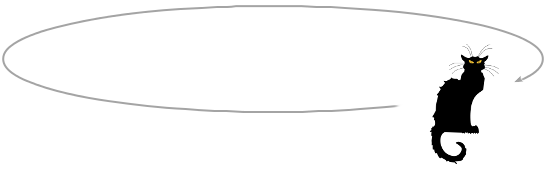
\includegraphics[width=8cm]{img/cat-animation.png}
\vskip 1.5ex\index{top (CSS)}\index{left (CSS)}\index{centering}\index{relative positioning}

Our picture is centered on the page and given a \lstinline`position` of \lstinline`relative`. We'll repeatedly update that picture's \lstinline`top` and \lstinline`left` styles to move it.\index{requestAnimationFrame function}\index{drawing}\index{animation}

\label{dom.animationFrame}The script uses \lstinline`requestAnimationFrame` to schedule the \lstinline`animate` function to run whenever the browser is ready to repaint the screen. The \lstinline`animate` function itself again calls \lstinline`requestAnimationFrame` to schedule the next update. When the browser window (or tab) is active, this will cause updates to happen at a rate of about 60 per second, which tends to produce a good-looking animation.\index{timeline}\index{blocking}

If we just updated the DOM in a loop, the page would freeze, and nothing would show up on the screen. Browsers do not update their display while a JavaScript program is running, nor do they allow any interaction with the page. This is why we need \lstinline`requestAnimationFrame`—it lets the browser know that we are done for now, and it can go ahead and do the things that browsers do, such as updating the screen and responding to user actions.\index{smooth animation}

The animation function is passed the current \index{time}time as an argument. To ensure that the motion of the cat per millisecond is stable, it bases the speed at which the angle changes on the difference between the current time and the last time the function ran. If it just moved the angle by a fixed amount per step, the motion would stutter if, for example, another heavy task running on the same computer were to prevent the function from running for a fraction of a second.\index{Math.cos function}\index{Math.sin function}\index{cosine}\index{sine}\index{trigonometry}

\label{dom.sin_cos}Moving in \index{circle}circles is done using the trigonometry functions \lstinline`Math.cos` and \lstinline`Math.sin`. For those who aren't familiar with these, I'll briefly introduce them since we will occasionally use them in this book.\index{coordinates}\index{pi}

\lstinline`Math.cos` and \lstinline`Math.sin` are useful for finding points that lie on a circle around point (0,0) with a radius of one. Both functions interpret their argument as the position on this circle, with zero denoting the point on the far right of the circle, going clockwise until 2π (about 6.28) has taken us around the whole circle. \lstinline`Math.cos` tells you the x-coordinate of the point that corresponds to the given position, and \lstinline`Math.sin` yields the y-coordinate. Positions (or angles) greater than 2π or less than 0 are valid—the rotation repeats so that \emph{a}+2π refers to the same \index{angle}angle as \emph{a}.\index{PI constant}

This unit for measuring angles is called \index{radian}radians—a full circle is 2π radians, similar to how it is 360 degrees when measuring in degrees. The constant π is available as \lstinline`Math.PI` in JavaScript.

\vskip 1.5ex
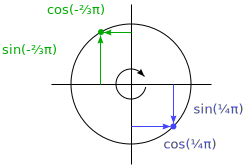
\includegraphics[width=6cm]{img/generated/cos_sin.pdf}
\vskip 1.5ex\index{counter variable}\index{Math.sin function}\index{top (CSS)}\index{Math.cos function}\index{left (CSS)}\index{ellipse}

The cat animation code keeps a counter, \lstinline`angle`, for the current angle of the animation and increments it every time the \lstinline`animate` function is called. It can then use this angle to compute the current position of the image element. The \lstinline`top` style is computed with \lstinline`Math.sin` and multiplied by 20, which is the vertical radius of our ellipse. The \lstinline`left` style is based on \lstinline`Math.cos` and multiplied by 200 so that the ellipse is much wider than it is high.\index{unit (CSS)}

Note that styles usually need \emph{units}. In this case, we have to append \lstinline`"px"` to the number to tell the browser that we are counting in \index{pixel}pixels (as opposed to centimeters, ``ems'', or other units). This is easy to forget. Using numbers without units will result in your style being ignored—unless the number is 0, which always means the same thing, regardless of its unit.

\section{Summary}

JavaScript programs may inspect and interfere with the document that the browser is displaying through a data structure called the DOM. This data structure represents the browser's model of the document, and a JavaScript program can modify it to change the visible document.

The DOM is organized like a tree, in which elements are arranged hierarchically according to the structure of the document. The objects representing elements have properties such as \lstinline`parentNode` and \lstinline`childNodes`, which can be used to navigate through this tree.

The way a document is displayed can be influenced by \emph{styling}, both by attaching styles to nodes directly and by defining rules that match certain nodes. There are many different style properties, such as \lstinline`color` or \lstinline`display`. JavaScript code can manipulate an element's style directly through its \lstinline`style` property.

\section{Exercises}

\label{dom.exercise_table}\subsection{Build a table}\index{table (HTML tag)}

An HTML table is built with the following tag structure:

\begin{lstlisting}
<table>
  <tr>
    <th>name</th>
    <th>height</th>
    <th>place</th>
  </tr>
  <tr>
    <td>Kilimanjaro</td>
    <td>5895</td>
    <td>Tanzania</td>
  </tr>
</table>
\end{lstlisting}
\noindent\index{tr (HTML tag)}\index{th (HTML tag)}\index{td (HTML tag)}

For each \emph{\index{row}row}, the \lstinline`<table>` tag contains a \lstinline`<tr>` tag. Inside of these \lstinline`<tr>` tags, we can put cell elements: either heading cells (\lstinline`<th>`) or regular cells (\lstinline`<td>`).

Given a data set of mountains, an array of objects with \lstinline`name`, \lstinline`height`, and \lstinline`place` properties, generate the DOM structure for a table that enumerates the objects. It should have one column per key and one row per object, plus a header row with \lstinline`<th>` elements at the top, listing the column names.

Write this so that the columns are automatically derived from the objects, by taking the property names of the first object in the data.

Add the resulting table to the element with an \lstinline`id` attribute of \lstinline`"mountains"` so that it becomes visible in the document.\index{right-aligning}\index{text-align (CSS)}

Once you have this working, right-align cells that contain number values by setting their \lstinline`style.textAlign` property to \lstinline`"right"`.

\subsection{Elements by tag name}\index{getElementsByTagName method}\index{recursion}

The \lstinline`document.getElementsByTagName` method returns all child elements with a given tag name. Implement your own version of this as a function that takes a node and a string (the tag name) as arguments and returns an array containing all descendant element nodes with the given tag name.\index{nodeName property}\index{capitalization}\index{toLowerCase method}\index{toUpperCase method}

To find the tag name of an element, use its \lstinline`nodeName` property. But note that this will return the tag name in all uppercase. Use the \lstinline`toLowerCase` or \lstinline`toUpperCase` string methods to compensate for this.

\subsection{The cat's hat}\index{cat's hat (exercise)}\index{animation!spinning cat}

Extend the cat animation defined \hyperref[dom.animation]{earlier} so that both the cat and his hat (\lstinline`<img src="img/hat.png">`) orbit at opposite sides of the ellipse.

Or make the hat circle around the cat. Or alter the animation in some other interesting way.\index{absolute positioning}\index{top (CSS)}\index{left (CSS)}\index{position (CSS)}

To make positioning multiple objects easier, it is probably a good idea to switch to absolute positioning. This means that \lstinline`top` and \lstinline`left` are counted relative to the top left of the document. To avoid using negative coordinates, which would cause the image to move outside of the visible page, you can add a fixed number of pixels to the position values.
